\documentclass[11pt]{beamer}
\usepackage[utf8]{inputenc}
\usepackage[T1]{fontenc}

\usepackage[backend=bibtex,style=authoryear]{biblatex}
\addbibresource{brownbags.bib}

%% End of citations additions

%\usetheme{AnnArbor}
%\usetheme{Antibes}
%\usetheme{Berkeley}
%\usetheme{Berlin}
%\usetheme{boxes}
%\usetheme{Darmstadt}
%\usetheme{default}
%\usetheme{Frankfurt}
%\usetheme{Ilmenau}
%\usetheme{JuanLesPins}
\usetheme{Luebeck}
%\usetheme{Malmoe}
%\usetheme{Montpellier}
%\usetheme{PaloAlto}
%\usetheme{Rochester}
%\usetheme{Singapore}
%\usetheme{Szeged}
%\hypersetup{
%	colorlinks=true,
%	linkcolor=blue,
%	filecolor=magenta,      
%	urlcolor=cyan,
%}

\setbeamertemplate{footline}
{%
	\leavevmode%
	\hbox{\begin{beamercolorbox}[wd=.2\paperwidth,ht=2.5ex,dp=1.125ex,leftskip=.3cm,rightskip=.3cm plus1fill]{author in head/foot}%
			\usebeamerfont{author in head/foot} \insertframenumber{} / \inserttotalframenumber
		\end{beamercolorbox}%
		\begin{beamercolorbox}[wd=.3\paperwidth,ht=2.5ex,dp=1.125ex,leftskip=.3cm plus1fill,rightskip=.3cm]{author in head/foot}%
			\usebeamerfont{author in head/foot}\insertshortauthor
		\end{beamercolorbox}%
		\begin{beamercolorbox}[wd=.5\paperwidth,ht=2.5ex,dp=1.125ex,leftskip=.3cm,rightskip=.3cm plus1fil]{title in head/foot}%
			\usebeamerfont{title in head/foot}\insertshorttitle
	\end{beamercolorbox}}%
	\vskip0pt%
}
\setbeamertemplate{headline}{}

\begin{document}
	\author{Gary R Seamans}
	\title{Statistical Inference}
	\subtitle{R Brown Bag Series \#5}
	%\logo{\scalebox{0.035}{
\includegraphics{R_logo.png}}}
	\institute{The MITRE Corporation}
	%\date{}
	%\subject{}
	%\setbeamercovered{transparent}
	%\setbeamertemplate{navigation symbols}{}
	\begin{frame}[plain]
		\maketitle
    \end{frame}

\begin{frame}{
	\begin{minipage}[t]{0.55\textwidth}
		Agenda
	\end{minipage}
	\hfill
	\begin{minipage}[t]{0.35\textwidth}
		\flushright
		\scalebox{0.035}{
\includegraphics{R_logo.png}}
	\end{minipage}
}{}
%% ==================== Content ===========================%%
\begin{center}
	\begin{itemize}
		\item Overview
		\item Discussion
		\item Questions
	\end{itemize}
\end{center}
\end{frame}

%% Tools ===================
\begin{frame}{
	\begin{minipage}[t]{0.55\textwidth}
		Overview
	\end{minipage}
	\hfill
	\begin{minipage}[t]{0.35\textwidth}
		\flushright
		\scalebox{0.035}{
\includegraphics{R_logo.png}}
	\end{minipage}
}{}
%% ==================== Content ===========================%%

Statistical inference can be defined: \textit{"...as the process of generating conclusions about a population from a noisy sample."} \parencite{CaffoStatisticalinferencedata2016}

\begin{center}
	\scalebox{0.08}{
\includegraphics{inference.png}}
\end{center}
\end{frame}
%% Concerns ===================
\begin{frame}{
	\begin{minipage}[t]{0.55\textwidth}
		Concerns
	\end{minipage}
	\hfill
	\begin{minipage}[t]{0.35\textwidth}
		\flushright
		\scalebox{0.035}{
\includegraphics{R_logo.png}}
	\end{minipage}
}{}
%% ==================== Content ===========================%%
\begin{itemize}
	\item Representative sample
	\item Contamination
	\item Bias
	\item Randomness
\end{itemize}
\end{frame}

%% Concerns ===================
\begin{frame}{
	\begin{minipage}[t]{0.55\textwidth}
		Concerns Example
	\end{minipage}
	\hfill
	\begin{minipage}[t]{0.35\textwidth}
		\flushright
		\scalebox{0.035}{
\includegraphics{R_logo.png}}
	\end{minipage}
}{}
%% ==================== Content ===========================%%
The China Study is a well known study that claims, among other  things, that animal protein is the primary cause of many illnesses, including cancer and heart disease.

\vspace{0.3cm}
Critics claim that the China study exhibits pretty much everything that can done wrong in a study. Without taking sides it is an interesting example. The back and forth between Dr. Campbell and his critics can be illuminating.

\vspace{0.3cm}
Starting Points:

\vspace{0.3cm}
China Study \parencite{CampbellChinaStudy1968}

\vspace{0.3cm}
Rebuttal \parencite{WhatDrCampbell}
\end{frame}

%% Goals ===================
\begin{frame}{
	\begin{minipage}[t]{0.55\textwidth}
		Goals
	\end{minipage}
	\hfill
	\begin{minipage}[t]{0.35\textwidth}
		\flushright
		\scalebox{0.035}{
\includegraphics{R_logo.png}}
	\end{minipage}
}{}
%% ==================== Content ===========================%%
\begin{itemize}
	\item Estimate and Quantify
	\item Is it a benchmark value?
	\item Mechanistic relationship
	\item Policy impact
	\item Probability of occurrence
\end{itemize}
\end{frame}



%% Tools ===================
\begin{frame}{
	\begin{minipage}[t]{0.55\textwidth}
		Tools
	\end{minipage}
	\hfill
	\begin{minipage}[t]{0.35\textwidth}
		\flushright
		\scalebox{0.035}{
\includegraphics{R_logo.png}}
	\end{minipage}
}{}
%% ==================== Content ===========================%%
\begin{itemize}
	\item Randomization
	\item Random sampling
	\item Sampling models
	\item Hypothesis testing
	\item Confidence intervals
	\item Study design
	\item Nonparametric bootstrapping
	\item Permutation
	
\end{itemize}
\end{frame}

%% Styles ===================
\begin{frame}{
	\begin{minipage}[t]{0.55\textwidth}
		Styles
	\end{minipage}
	\hfill
	\begin{minipage}[t]{0.35\textwidth}
		\flushright
		\scalebox{0.035}{
\includegraphics{R_logo.png}}
	\end{minipage}
}{}
%% ==================== Content ===========================%%
\begin{itemize}
	\item Frequency probability and inference
	\item Bayesian probability and inference
\end{itemize}
\end{frame}

\usebackgroundtemplate{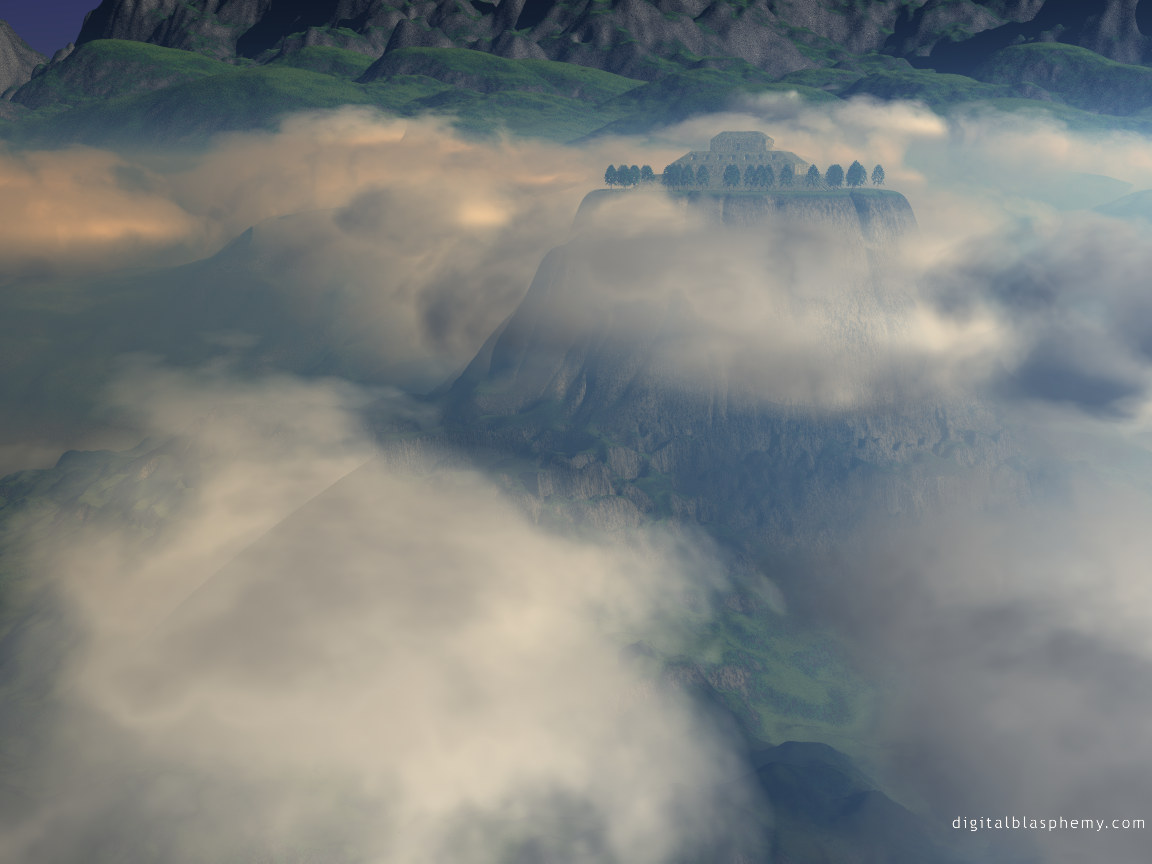
\includegraphics[width=\paperwidth, height=\paperheight]{nimbus.jpg}}
%% Bayesian ===================
\begin{frame}{
	\begin{minipage}[t]{0.55\textwidth}
		Bayesian
	\end{minipage}
	\hfill
	\begin{minipage}[t]{0.35\textwidth}
		\flushright
		\scalebox{0.035}{
\includegraphics{R_logo.png}}
	\end{minipage}
}{}
%% ==================== Content ===========================%%

	The first case study is on-time arrival prediction for domestic flights. Prediction is not an exact science.
	\vspace{0.5cm}
	
	\textit{Ah. Then, I will try to make the best guess I can.} Spock - The Voyage Home

\end{frame}
\usebackgroundtemplate{}

\usebackgroundtemplate{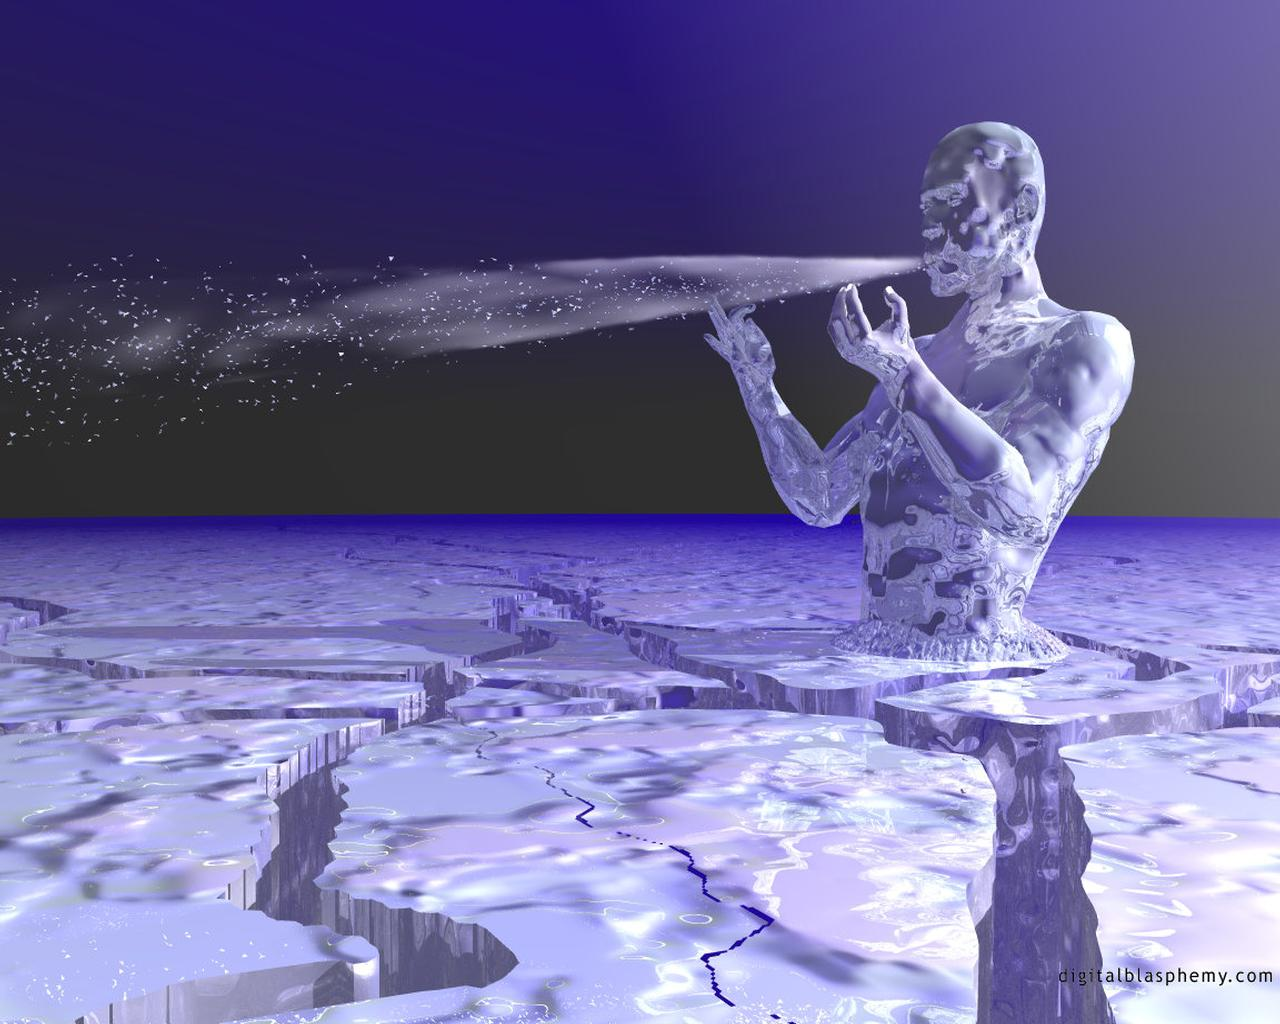
\includegraphics[width=\paperwidth, height=\paperheight]{frio_1280.jpg}}
%% Questions ===================
\begin{frame}{
	\begin{minipage}[t]{0.55\textwidth}
		Questions
	\end{minipage}
	\hfill
	\begin{minipage}[t]{0.35\textwidth}
		\flushright
		\scalebox{0.035}{
\includegraphics{R_logo.png}}
	\end{minipage}
}{}
%% ==================== Content ===========================%%
\begin{center}
	
\end{center}
\end{frame}

\usebackgroundtemplate{}

%%===================== Citations =================================%%
\appendix
\begin{frame}[allowframebreaks]{References}{}
\footnotesize
\printbibliography

\end{frame}
\end{document}